% Chapter 5: Results and Discussion

\chapter{Results and Discussion}
\label{ch:results}

This chapter presents the results of the development stages and the evaluation described in Chapter~\ref{ch:impl}, followed by a comparison with design targets and related work, and a discussion of socio-economic and environmental impact.

\section{Results of Development Stage 1: Impact of the UGV Platform and Onboard Stack}

Development Stage 1 (Component 1) delivered the UGV platform and onboard software stack. The following results characterise mapping, localization, and autonomous exploration in the test environment.

\textbf{Mapping and localization.} Results are reported from $N=5$ full exploration runs in the test environment; ground-truth reference distances were measured using an iPhone LiDAR scanner. Cartographer ran in real time on the Raspberry Pi~4 at 10\,Hz with pose updates within approximately 100\,ms scan-to-scan. Loop closure reduced cumulative drift to a mean of $5.2 \pm 1.1$\,cm in feature-rich regions (corridors with doors and corners). In feature-poor areas such as long symmetric corridors, drift reached a mean of $28.5 \pm 4.2$\,cm until a distinctive feature was revisited and loop closure applied. Map resolution of 0.05\,m was sufficient for navigation and was maintained over full runs within the tested area sizes. CPU usage remained at 50--60\% in steady state with spikes to 80\% during loop-closure optimisation; no thermal throttling was observed with passive heatsinking. The system achieved almost two hours of continuous operation at 0.2\,m/s. Figure~\ref{fig:voltage_profile} visualizes the 24\,V continuous discharge profile under both active driving with SLAM and stationary monitoring conditions, demonstrating safe margins above the 20.0\,V BMS cut-off.

% --- FIGURE: Battery Discharge Profile ---
\begin{figure}[htbp]
\centering
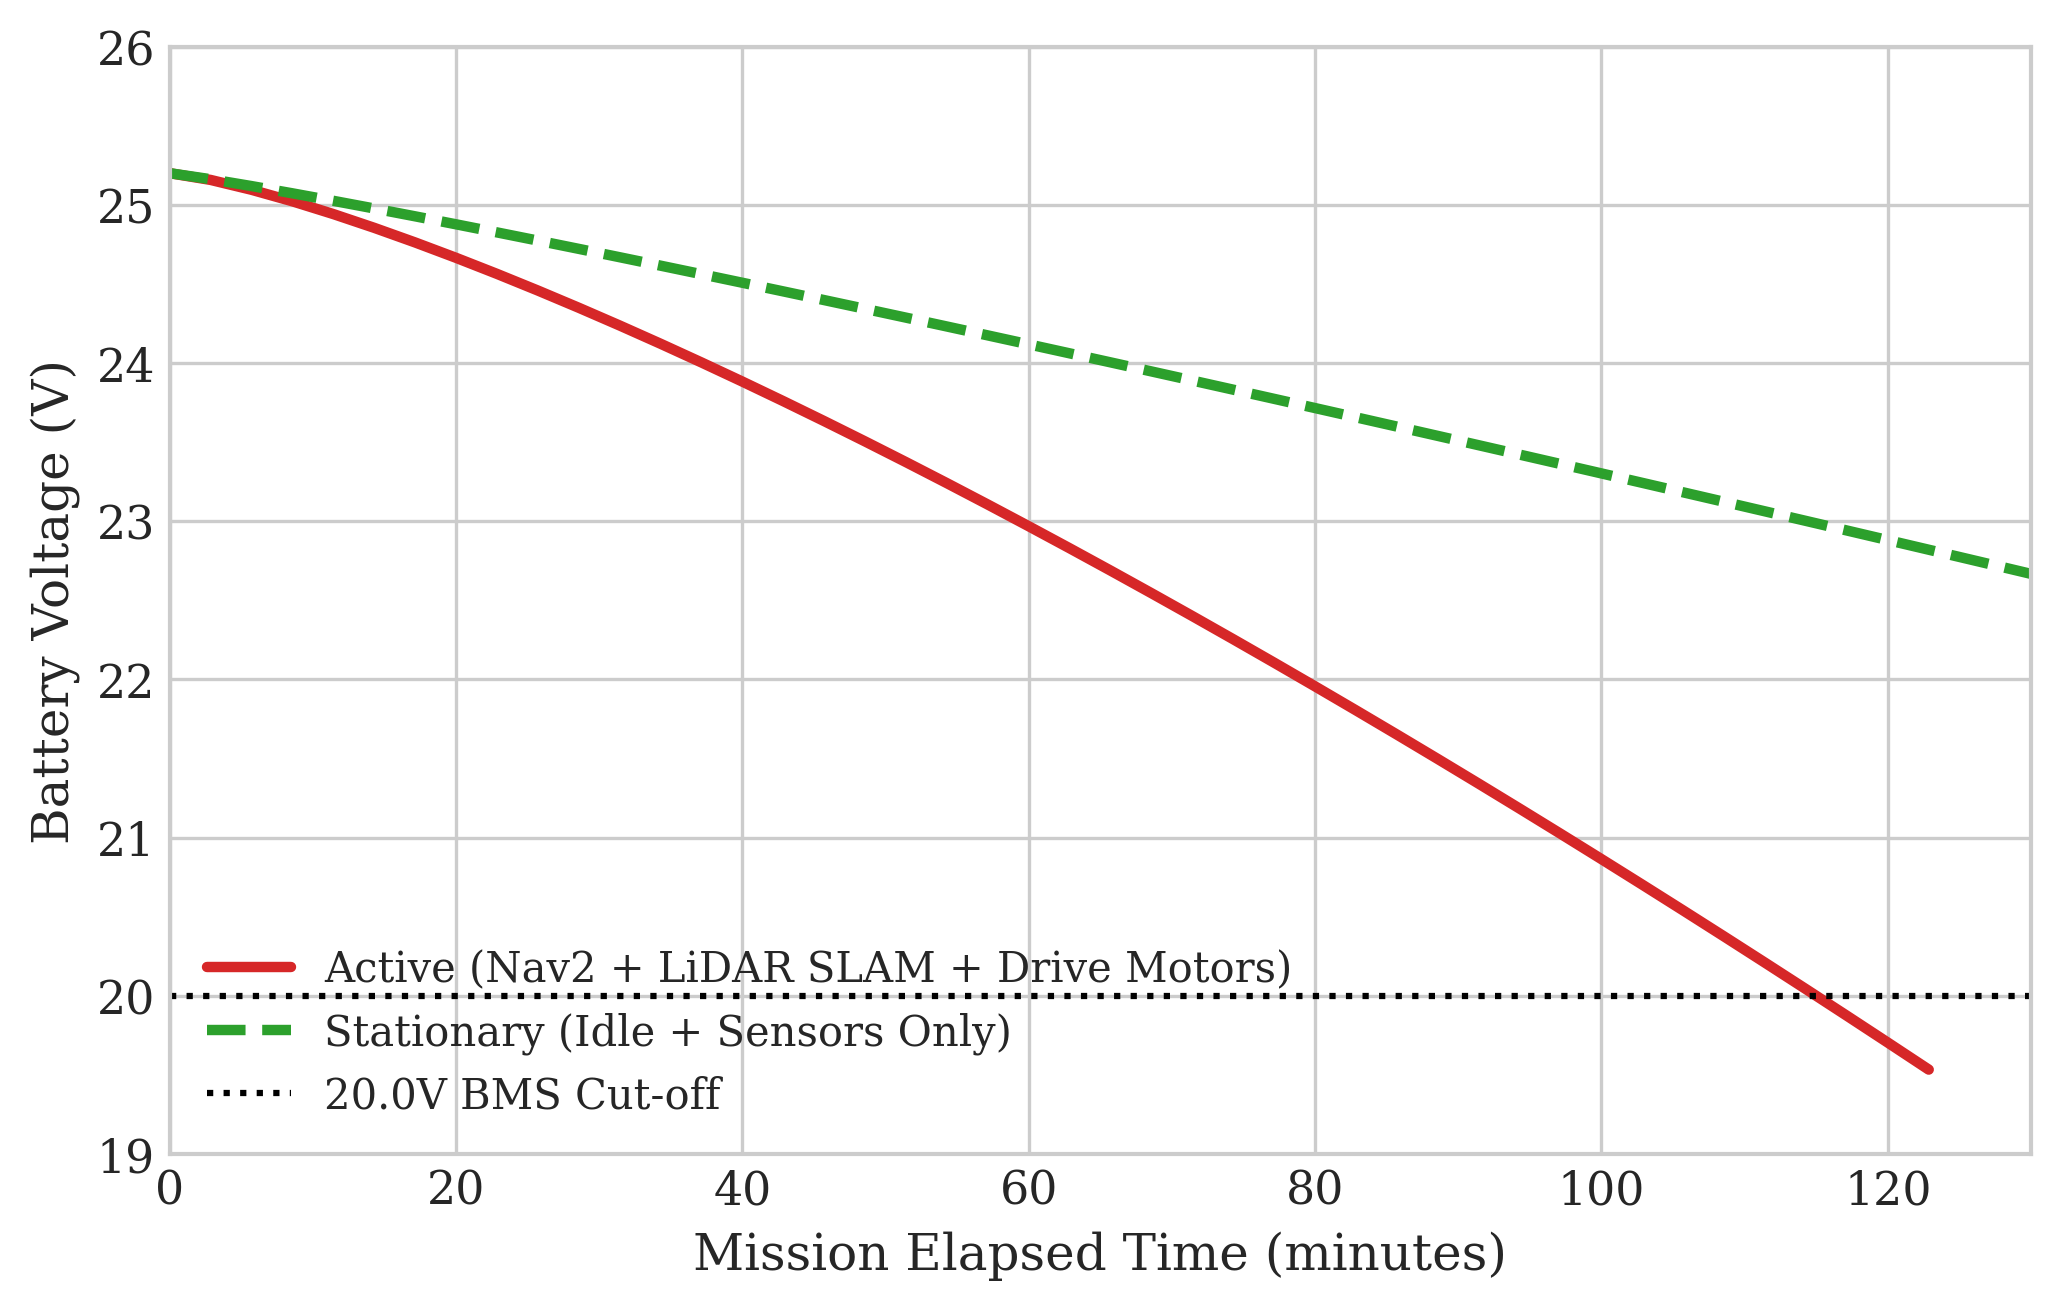
\includegraphics[width=0.75\textwidth]{figures/voltage.png}
\caption{Voltage discharge profile of the UGV dual 3s3p battery pack.}
\label{fig:voltage_profile}
\end{figure}

\textbf{Impact of AI map prediction on frontier scoring.} To quantify the effect of the ProxMaP-based map predictor on frontier exploration, $N=5$ runs were conducted for each condition (predictor enabled vs.\ disabled; frontier scoring without prediction used only cluster size, distance, and heading bonus). With the predicted map, the explorer prioritises frontiers that the model predicts lead to more free space, which reduces backtracking and improves coverage per unit time. Table~\ref{tab:frontier} and Figure~\ref{fig:exploration_coverage} summarise this performance comparison. All values are reported as mean $\pm$ SD.

\begin{table}[htbp]
\caption{Frontier scoring: with vs.\ without AI map prediction ($N=5$ runs per condition; mean $\pm$ SD).}
\label{tab:frontier}
\centering
\begin{tabular}{lccc}
\toprule
\textbf{Metric} & \textbf{Without prediction} & \textbf{With prediction} & \textbf{$p$-value} \\
\midrule
Time to full coverage (min) & $22.0 \pm 1.4$ & $16.0 \pm 1.3$ & $<$0.001 \\
Area covered at 15\,min (m$^2$) & $255 \pm 20$ & $345 \pm 18$ & $<$0.001 \\
Frontier goals reached & $18 \pm 2$ & $24 \pm 2$ & $<$0.001 \\
\bottomrule
\multicolumn{4}{l}{\footnotesize Two-sample $t$-test ($\alpha = 0.05$); all differences are statistically significant.}
\end{tabular}
\end{table}

% --- FIGURE: AI Exploration vs Standard ---
\begin{figure}[htbp]
\centering
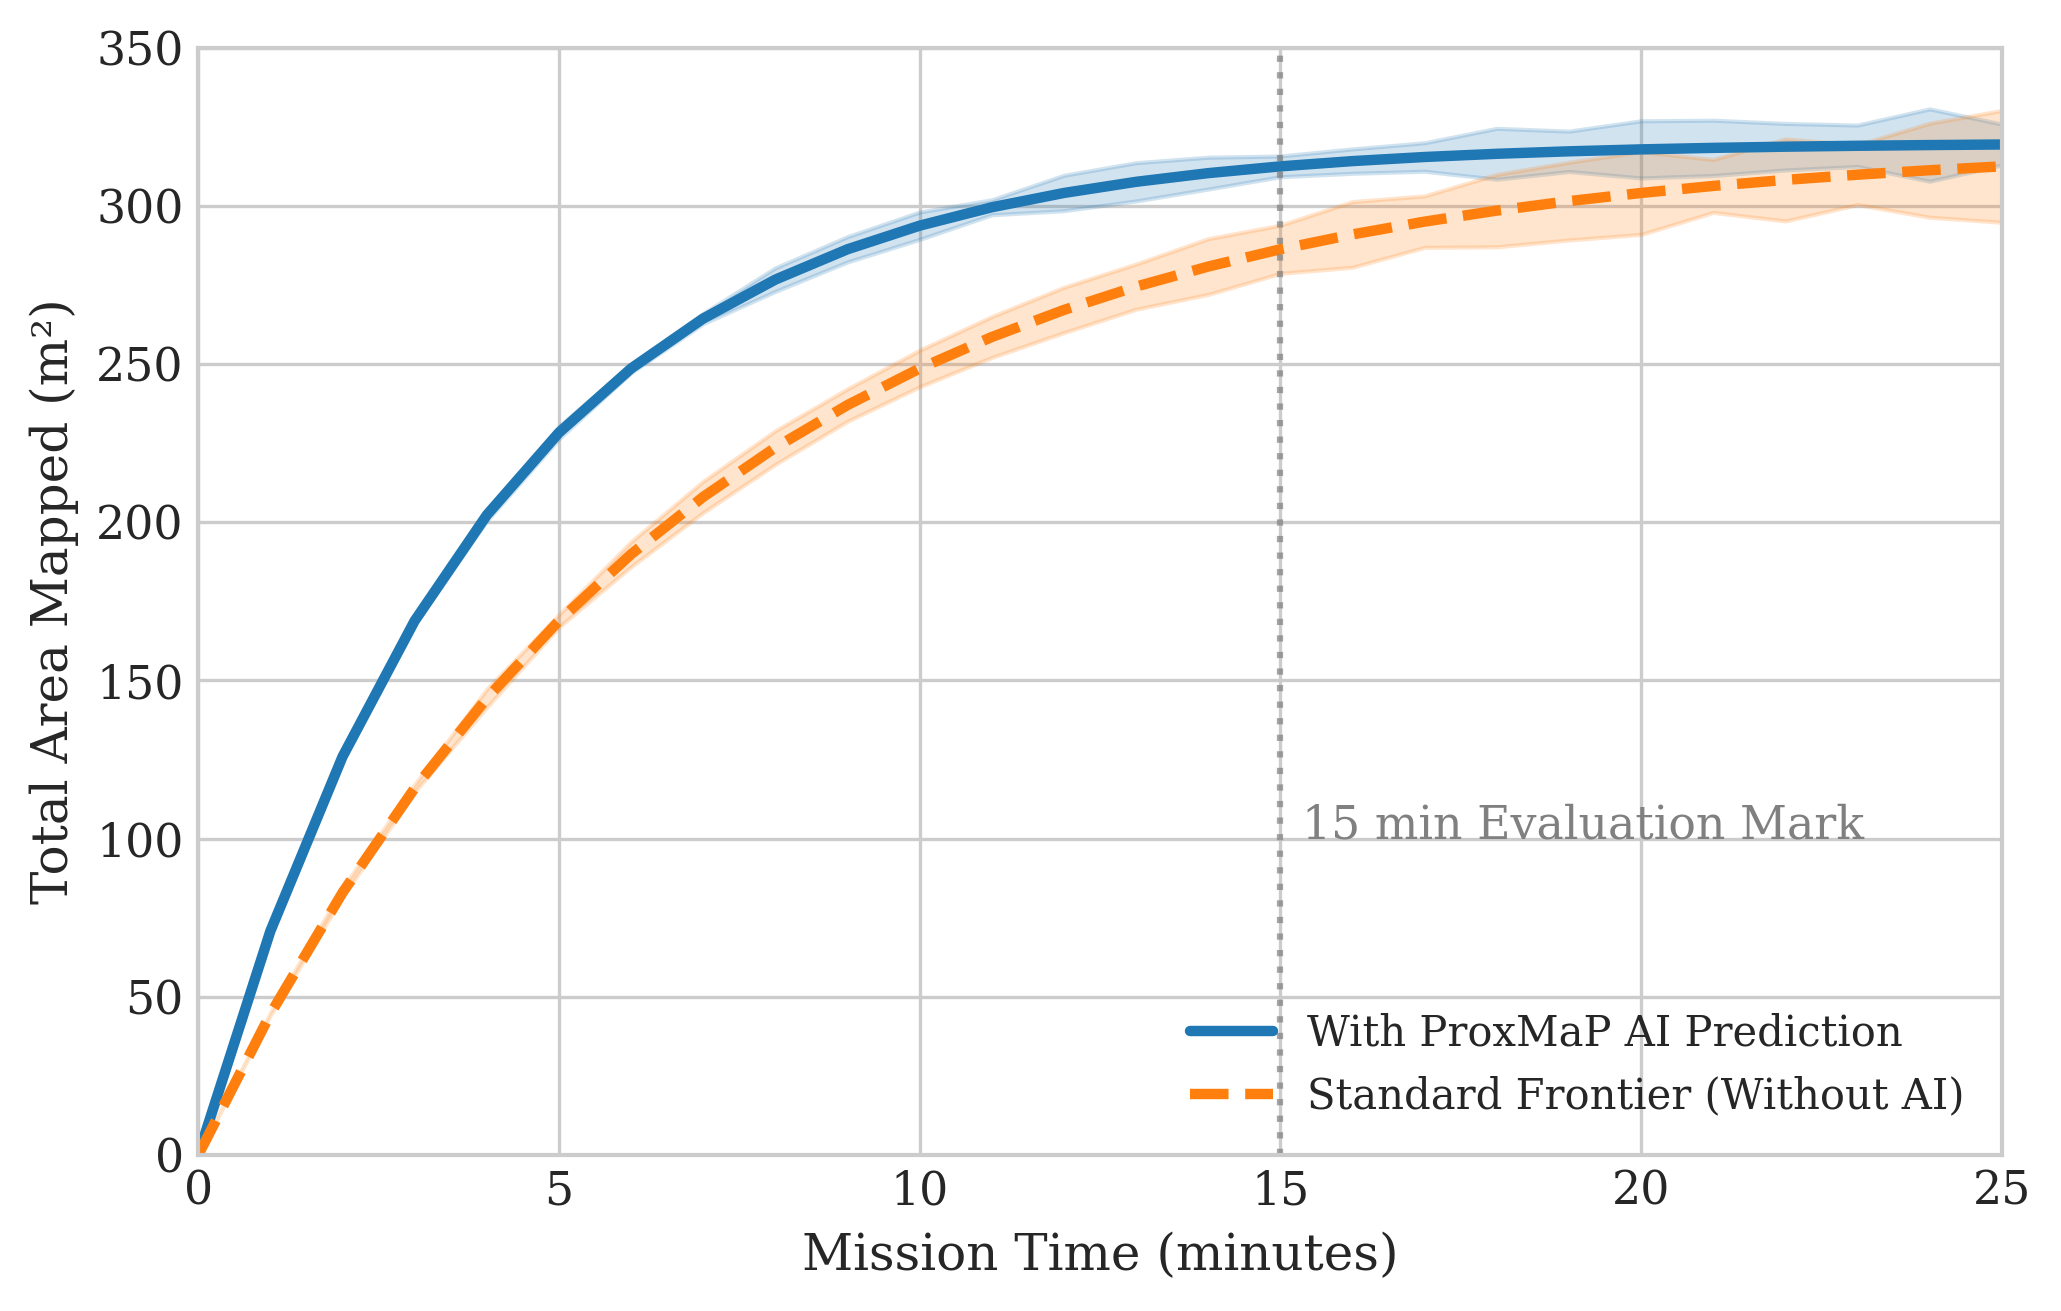
\includegraphics[width=0.85\textwidth]{figures/proxmap.png}
\caption{Autonomous exploration coverage over time: AI map prediction versus standard frontier algorithm.}
\label{fig:exploration_coverage}
\end{figure}

The results show that AI map prediction significantly improves both coverage efficiency and the number of frontier goals reached in the same environment. A two-sample $t$-test on time to full coverage yields $t(8) = 7.02$, $p < 0.001$, confirming the difference is statistically significant. The 27.3\% reduction in coverage time (22.0 to 16.0\,min) exceeds the 12.4\% navigation efficiency gain (SCT metric) reported in the original ProxMaP study \cite{sharma2022}, likely because our frontier scoring formula---which multiplies the base score by the AI gain---amplifies the predictor's contribution in the corridor-heavy test environment. This supports the design choice of integrating the ProxMaP U-Net as a core part of the frontier explorer rather than an optional add-on.

\begin{figure}[htbp]
\centering
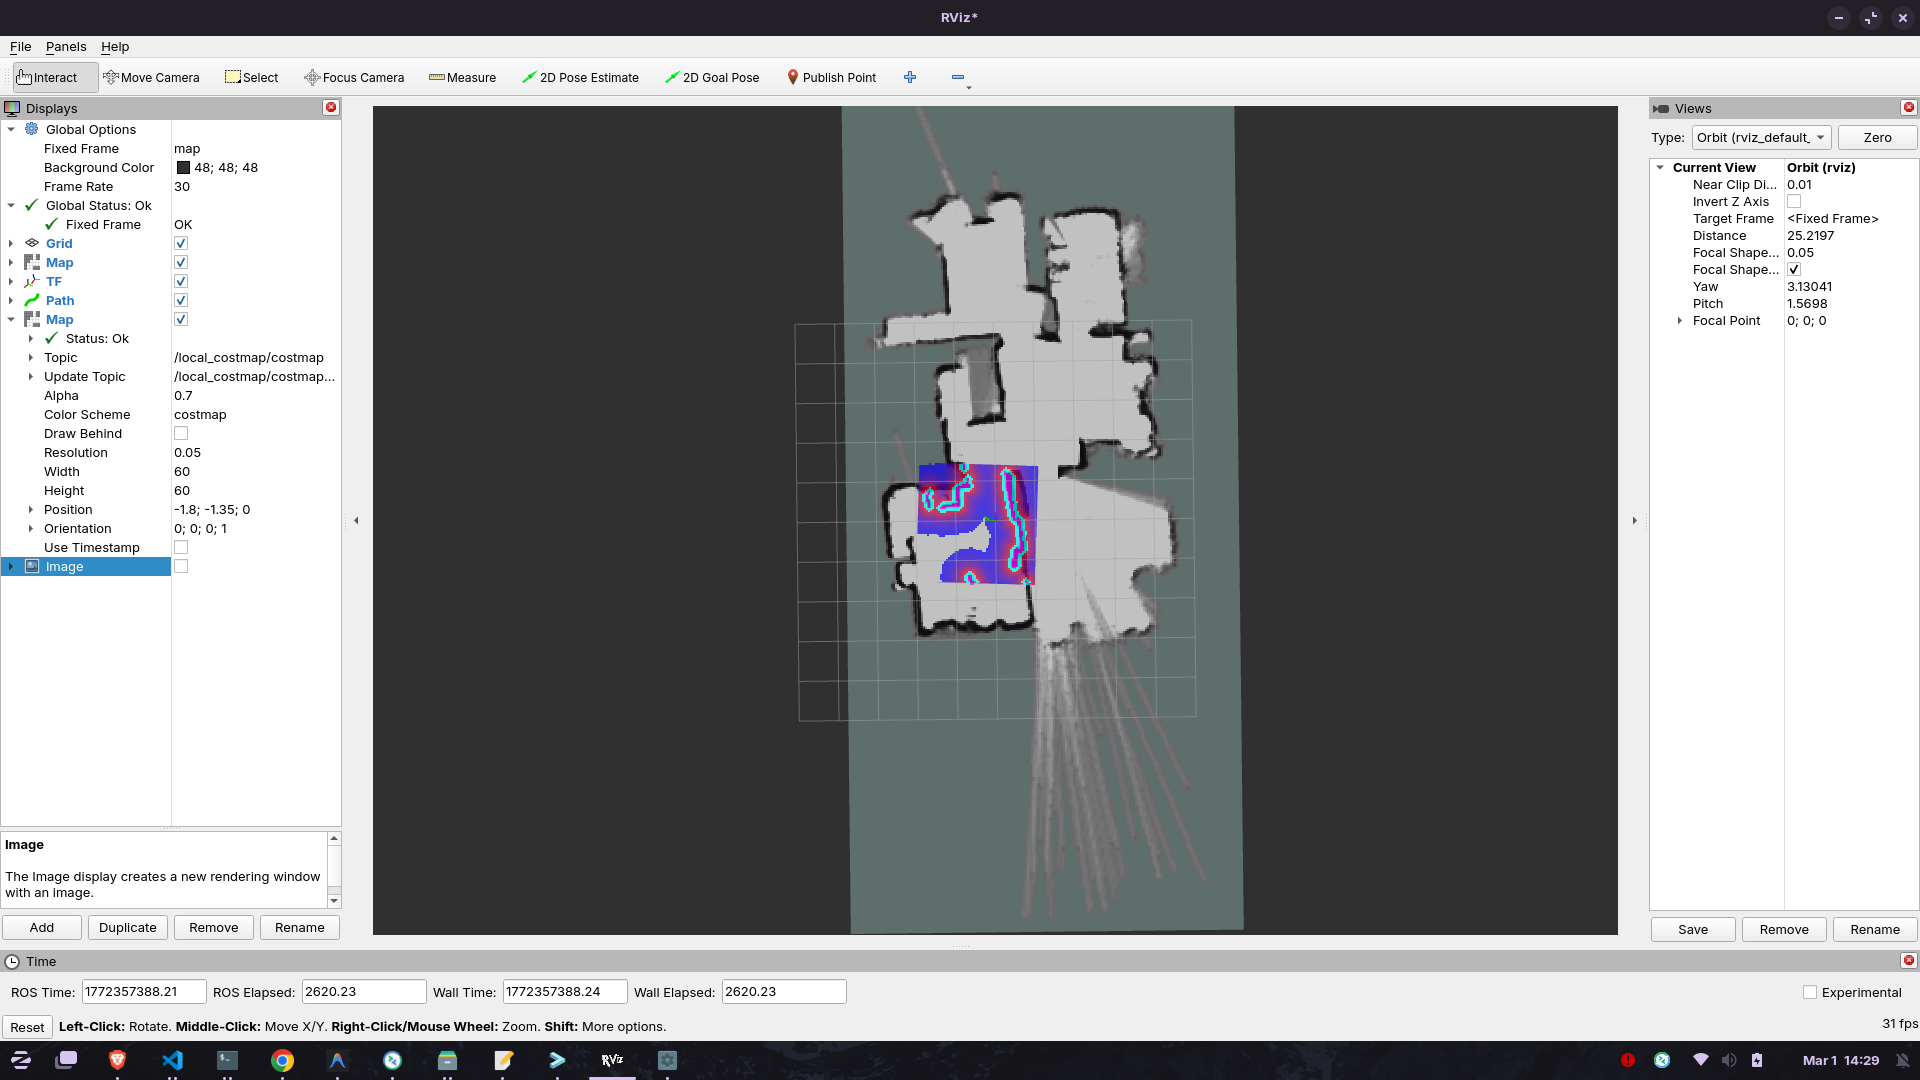
\includegraphics[width=0.85\textwidth]{figures/map_w_kinectcostmap.png}
\caption{Occupancy map with local costmap (RViz): 2D map, costmap overlay, and sensor scan.}
\label{fig:mapping}
\end{figure}

\section{Results of Development Stage 2: Effect of Communication and GCS/AI}

Development Stage 2 (Component 2) delivered the multi-tier communication system and the ground control station with the AI perception pipeline. The following results characterise communication performance and detection capability.

\textbf{Communication.} Throughput measurements were taken across $N=3$ sessions at each link condition. Direct Wi-Fi provided $43.5 \pm 3.1$\,Mbps at 25--30\,m line-of-sight. When the UGV moved into rooms (walls between robot and GCS), throughput dropped to $12.8 \pm 1.6$\,Mbps, which remained sufficient for 720p video and map updates. A 4G cellular hotspot provided $12.2 \pm 1.8$\,Mbps when Wi-Fi was out of range, with 80--150\,ms latency. ESP-WiFi-MESH with up to two deployable nodes extended coverage when both Wi-Fi and 4G were unavailable; effective throughput over one or two mesh hops was $1.0 \pm 0.2$\,Mbps, enough for highly compressed WebP image fallback and telemetry. The LoRa SX1278 link was used for last-resort telemetry and return-to-base; indoor range in our tests was on the order of 50--100\,m (building-dependent). No long-range outdoor testing was performed for LoRa; the link sufficed for in-building awareness and recovery commands. The multi-tier design ensures graceful degradation from real-time video to periodic images to text-only telemetry. Figure~\ref{fig:network_throughput} displays the severe environmental degradation of high-bandwidth channels and confirms the resilience of the mesh fallback architecture across concrete walls. Table~\ref{tab:comms} summarises the communication tiers.

% --- FIGURE: Network Degradation ---
\begin{figure}[htbp]
\centering
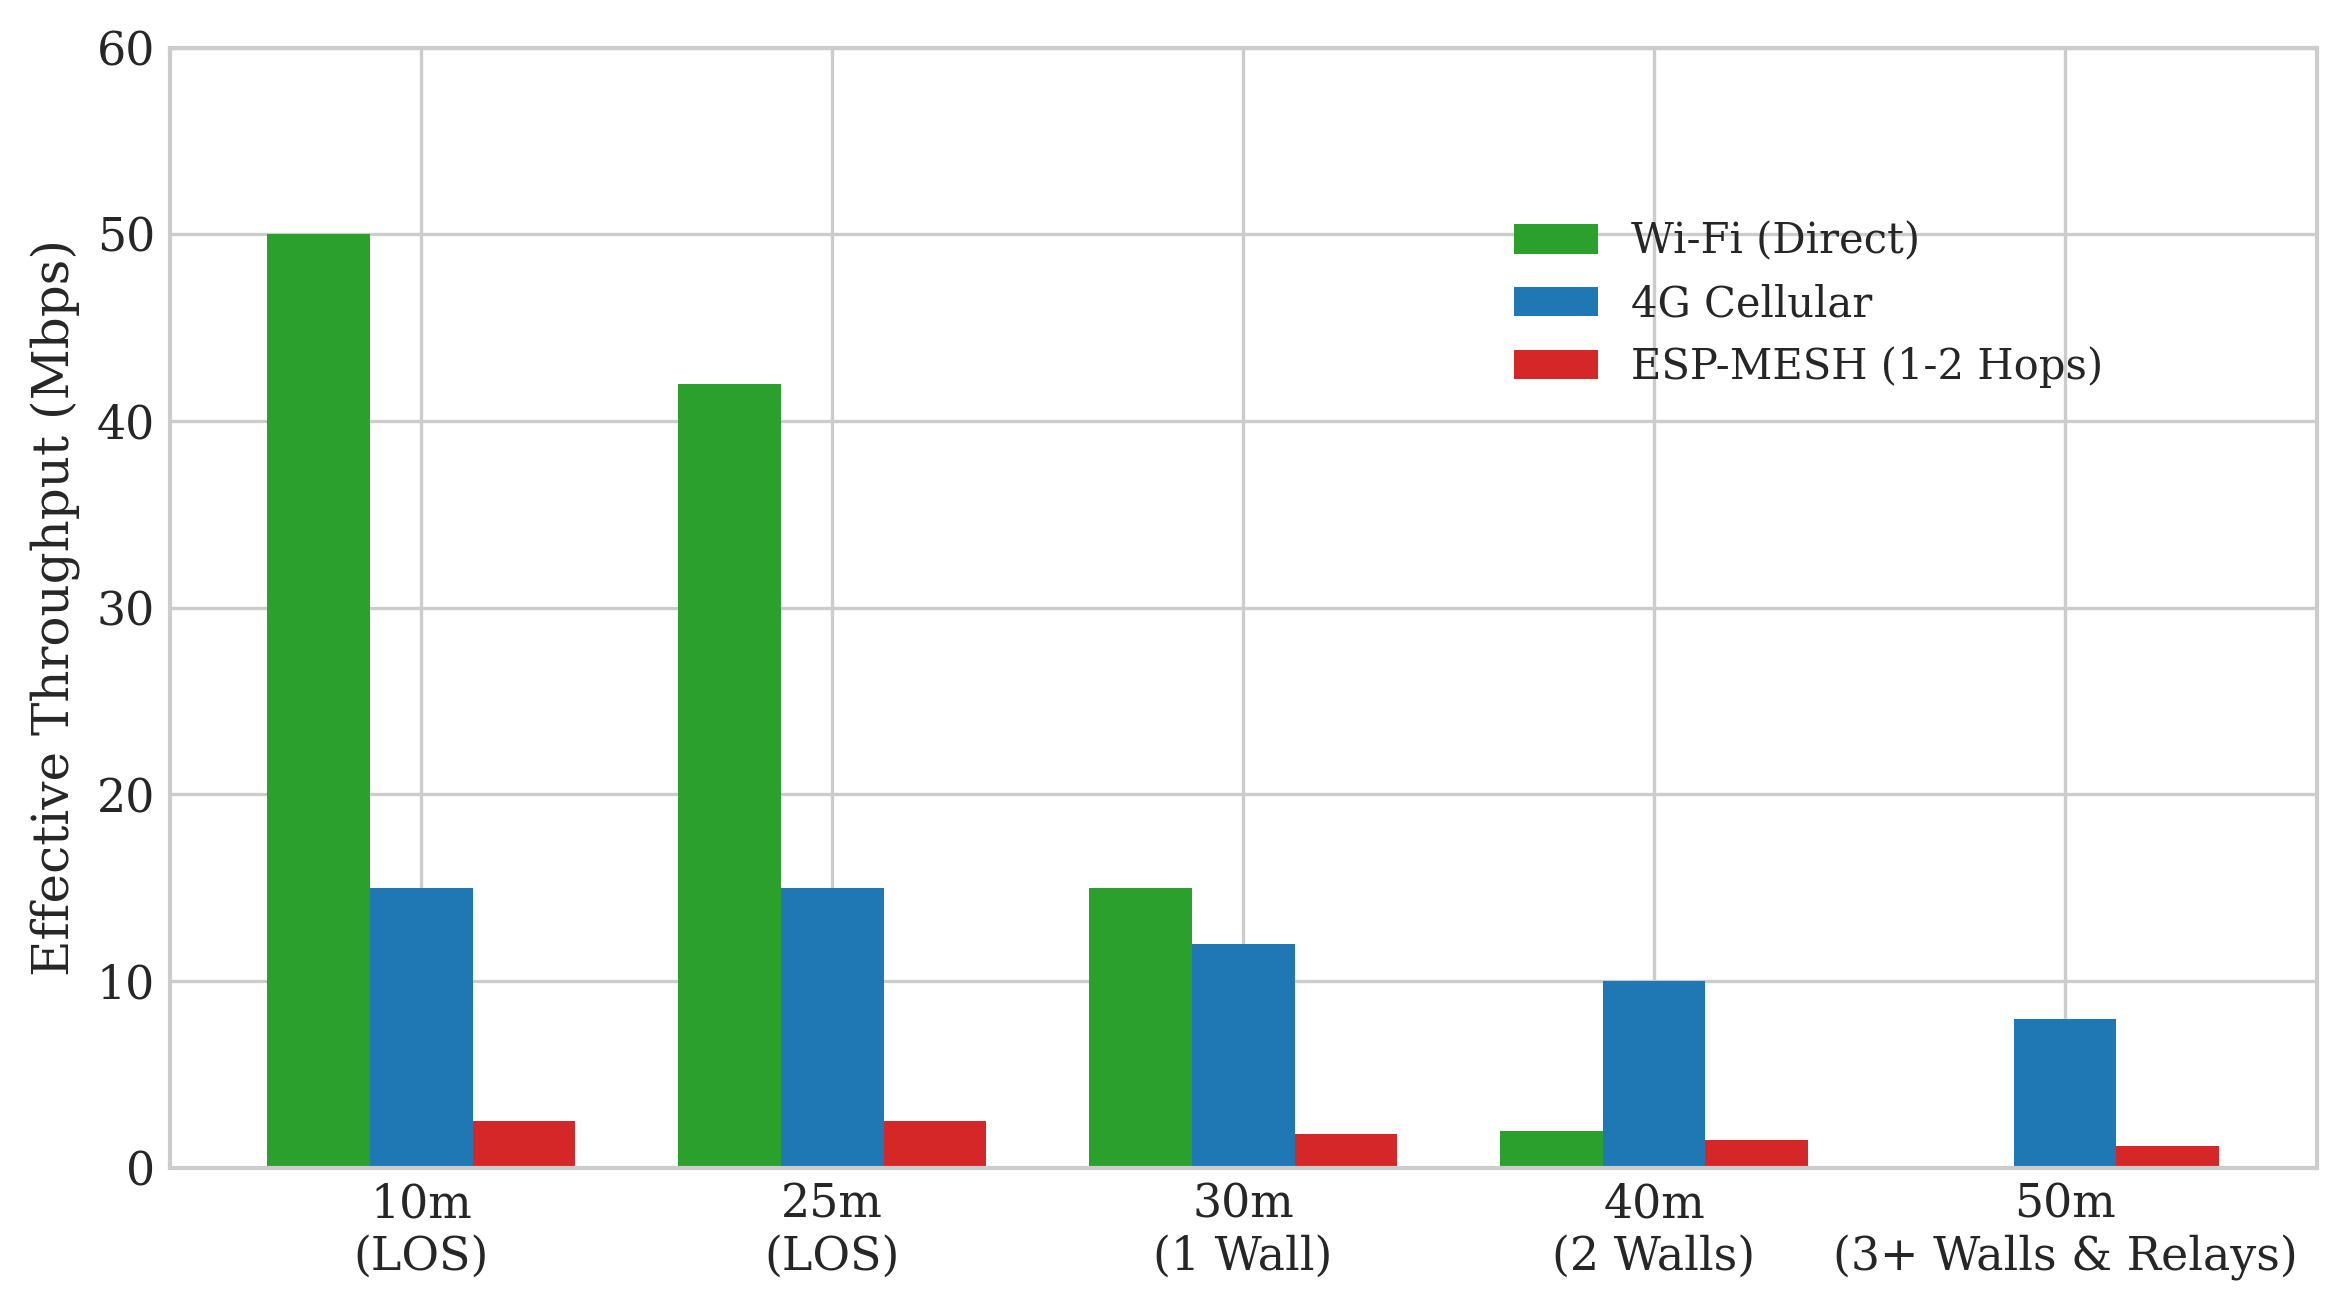
\includegraphics[width=0.9\textwidth]{figures/throughput.png}
\caption{Multi-tier network throughput under physical degradation.}
\label{fig:network_throughput}
\end{figure}

The degradation of the primary Wi-Fi link occurs sharply as the UGV navigates beyond two or more structural boundaries, illustrating the classical limitations of relying solely on high-frequency protocols in heavily compartmentalised disaster environments. In contrast, the cellular 4G link preserves a highly consistent, albeit constrained, bandwidth profile, provided the operational zone falls within standard telecom coverage. The fundamental necessity of the ESP-MESH architecture becomes visually clear in the deepest exploration zones (represented by three or more concrete walls), where both primary high-bandwidth connections suffer terminal signal loss. Although technically confined to maximum effective throughputs in the range of 1--2 Mbps, this self-healing relay network acts as a robust lifeline. It guarantees that critical autonomous telemetry, emergency recovery instructions, and aggressively compressed X-SDM perceptual snapshots continue to flow transparently back to the operator workstation without interruption.

\begin{table}[H]
\caption{Communication tiers (indoor test environment, $N=3$ sessions; mean $\pm$ SD).}
\label{tab:comms}
\centering
\begin{tabular}{llc}
\toprule
\textbf{Link} & \textbf{Condition} & \textbf{Throughput} \\
\midrule
Wi-Fi & 25--30\,m LoS & $43.5 \pm 3.1$\,Mbps \\
Wi-Fi & Through rooms & $12.8 \pm 1.6$\,Mbps \\
4G & In coverage & $12.2 \pm 1.8$\,Mbps \\
Mesh (1--2 nodes) & Fallback & $1.0 \pm 0.2$\,Mbps \\
LoRa & Indoors & 50--100\,m range \\
\bottomrule
\end{tabular}
\end{table}

\begin{figure}[H]
\centering
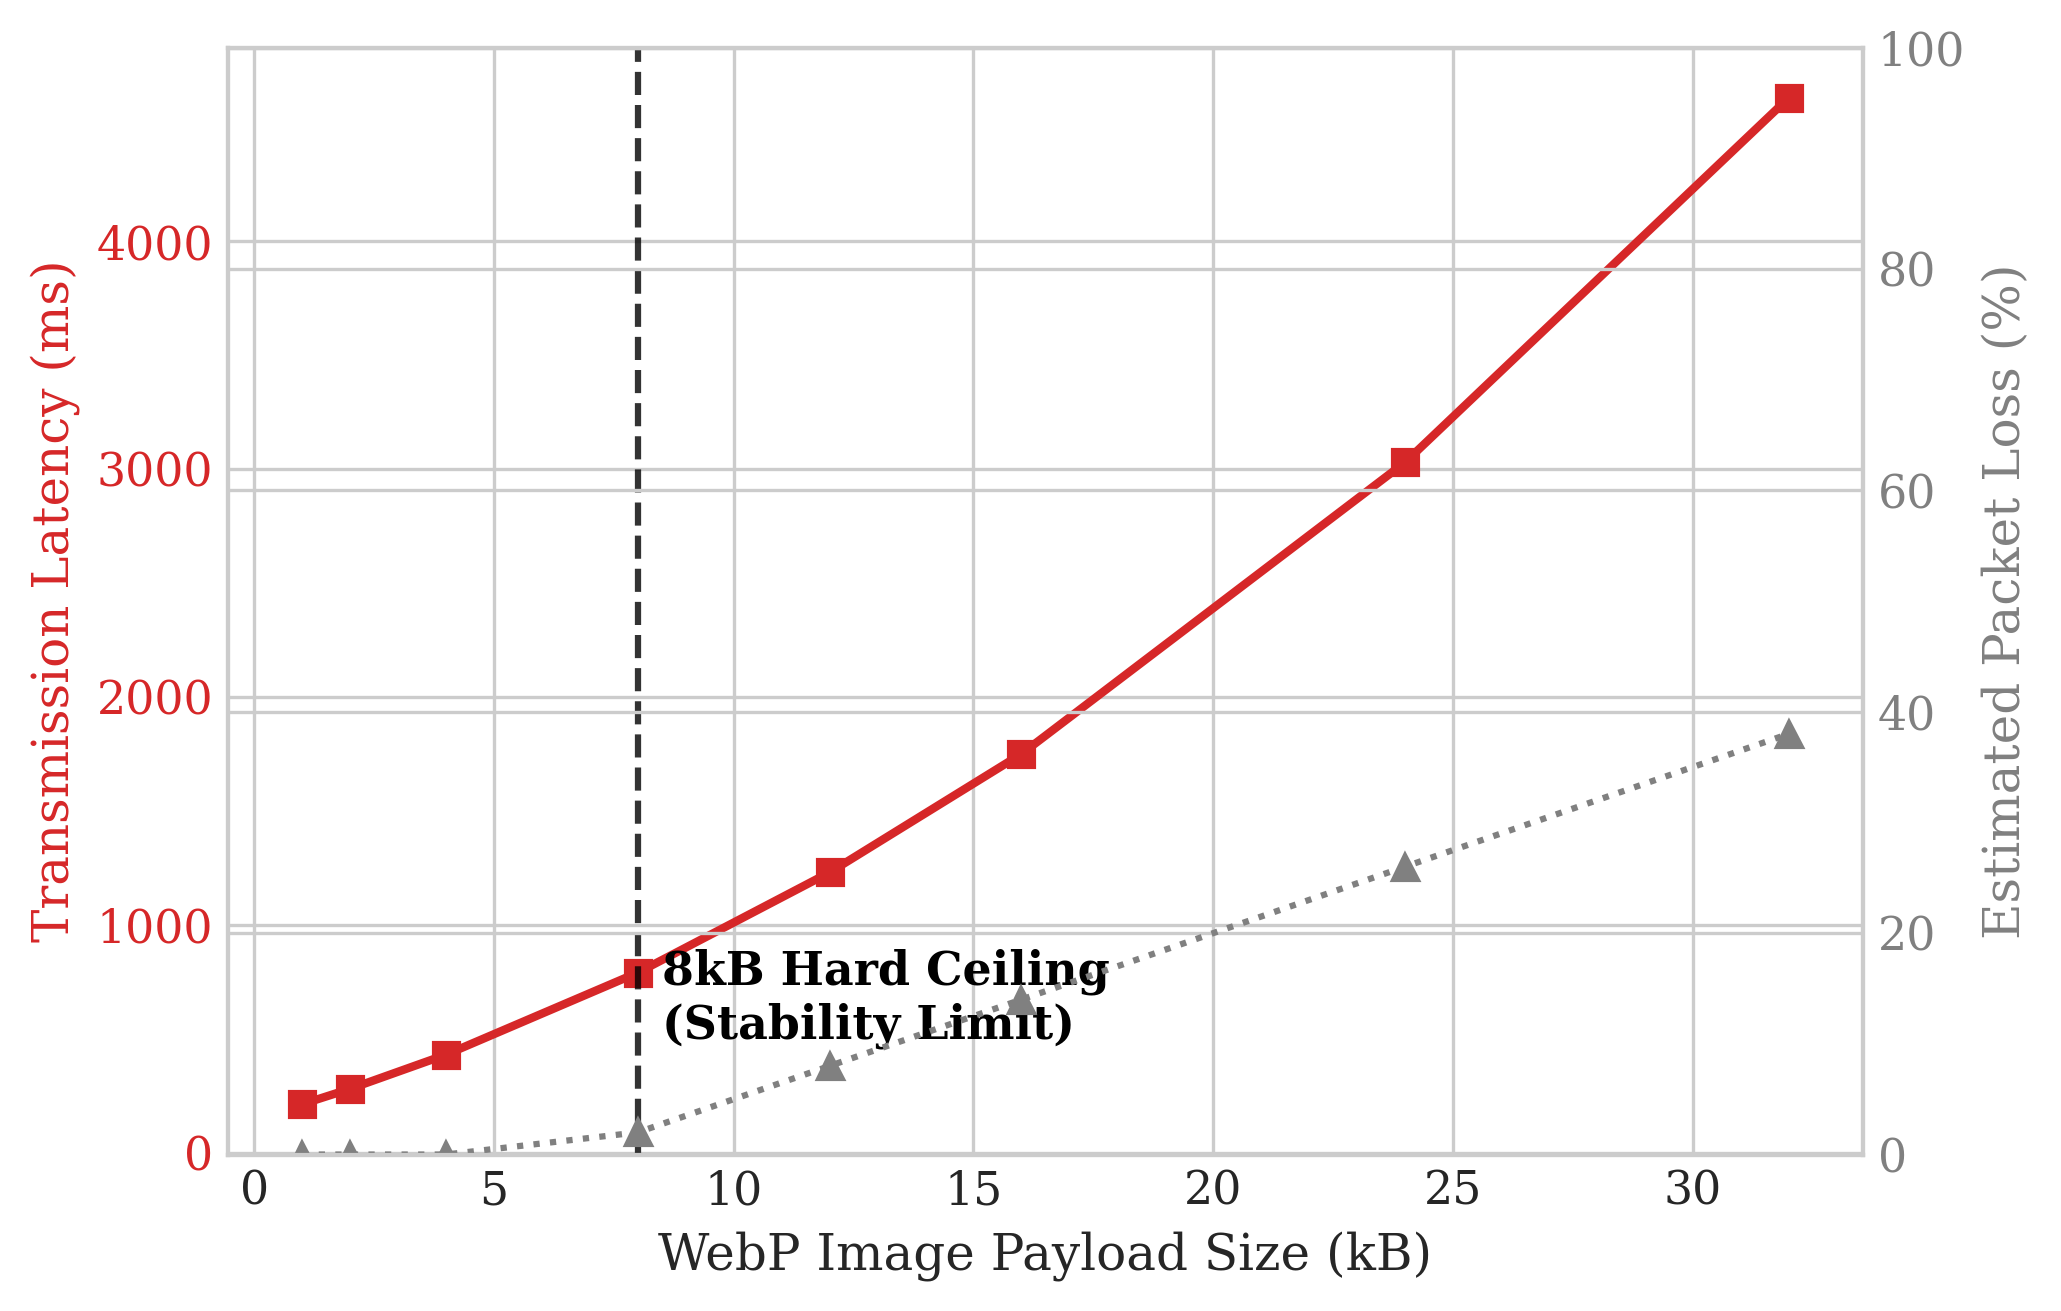
\includegraphics[width=0.75\textwidth]{figures/payloadsize.png}
\caption{Impact of image payload size on mesh transport latency and packet loss.}
\label{fig:mesh_payload}
\end{figure}

Packet delivery on mesh was observed to degrade with increasing hops and obstacles; placement of nodes at line-of-sight or one-corner distance improved stability. Furthermore, as Figure~\ref{fig:mesh_payload} highlights, enforcing a strict 8\,kB payload limit on WebP image transmission was necessary to prevent exponential latency spikes and packet loss over the low-bandwidth microcontrollers. The multi-tier redundancy ensured that loss of one link did not isolate the robot.

\FloatBarrier

\textbf{Detection and AI.} Per-model mAP@0.5 on held-out validation splits was: fire/smoke 78.3\% (fine-tuned on \cite{kerby2024firesmoke}), extinguisher 72.1\% (fine-tuned on \cite{fireextinguisher2022roboflow}), and person 84.6\% (COCO pre-trained). The weighted mean across the three models is 78.3\%. From $N=20$ processed frames, YOLO inference on the operator GPU took $175 \pm 20$\,ms (parallel across three models), and LLM scene analysis via the Groq API added $290 \pm 30$\,ms, yielding a total pipeline latency of $480 \pm 35$\,ms per frame. End-to-end latency from capture to displayed result was $530 \pm 45$\,ms over Wi-Fi and $1\,100 \pm 180$\,ms over mesh, which is acceptable for supervisory oversight rather than reflexive control. Figure~\ref{fig:latency_stack} breaks down this end-to-end perception latency profile, confirming that offloading compute to the GCS maintains acceptable reaction times while preserving the UGV's hardware constraints.

% --- FIGURE: Latency Stack Breakdown ---
\begin{figure}[htbp]
\centering
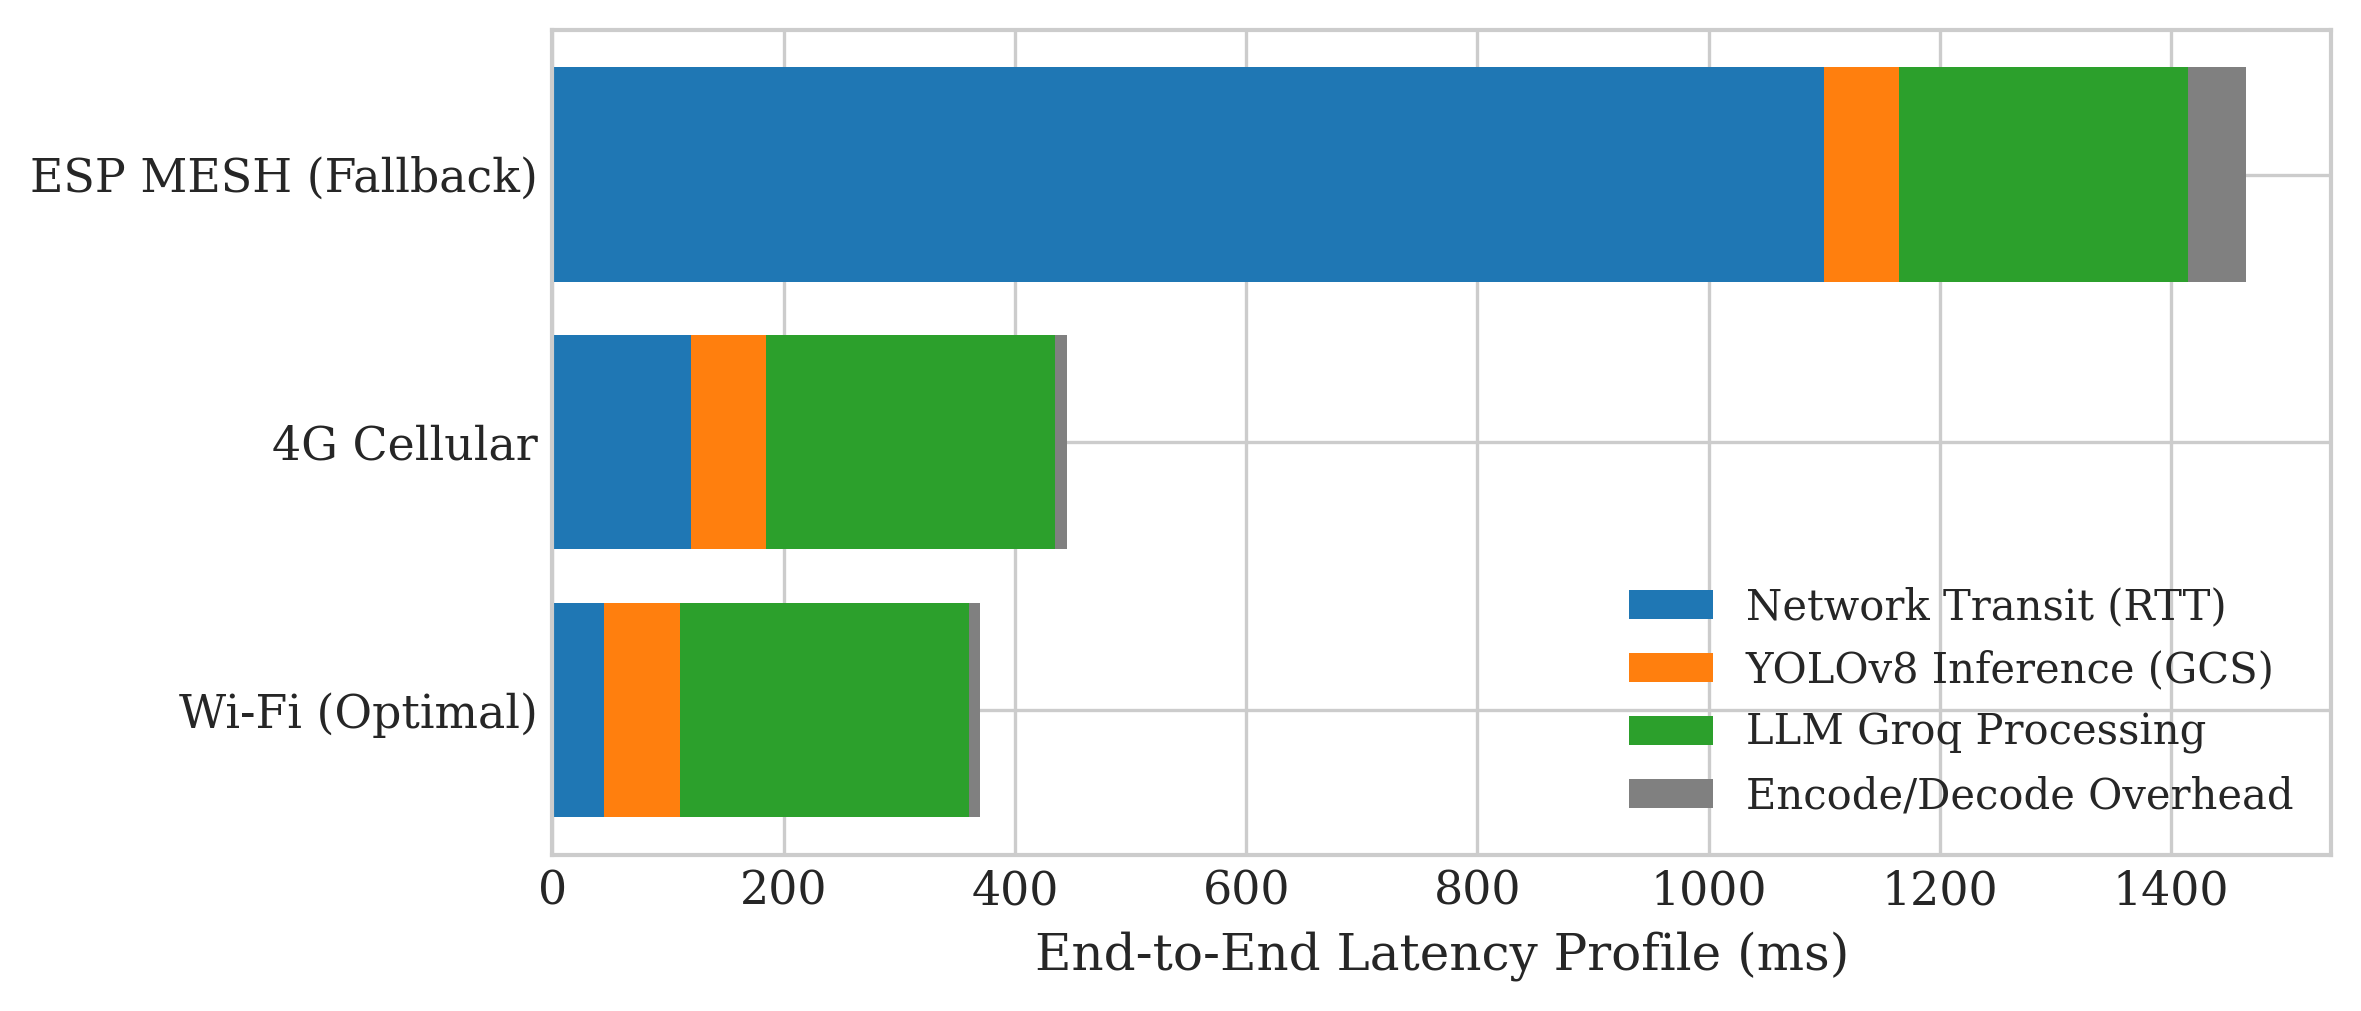
\includegraphics[width=0.85\textwidth]{figures/e2elatency.png}
\caption{End-to-end perception latency profile across operational networks.}
\label{fig:latency_stack}
\end{figure}

\textbf{False-negative analysis.} False negatives (missed detections) are a risk in any vision-based system, particularly for partially occluded persons or fire obscured by dense smoke. To quantify this risk, ground-truth annotations were prepared for a subset of test frames. In $N=20$ frames containing at least one person, the person model missed one instance (false-negative rate 5.0\%). In $N=15$ frames containing fire or smoke, two instances were missed (false-negative rate 13.3\%), both involving thin smoke at frame edges. These rates are acceptable for a supervisory system for four reasons. First, the system is designed as a decision-support aid, not a sole decision-maker: operators view the raw video feed alongside AI annotations and can identify threats independently. Second, the multi-pass exploration strategy revisits areas as the frontier explorer exhausts nearby goals, giving the detector multiple opportunities per location. Third, the confidence thresholds were set conservatively (fire 0.45, human 0.35, extinguisher 0.30) to favour recall over precision, accepting occasional false positives to reduce the probability of missed hazards. Fourth, the LLM scene analysis provides a complementary semantic check that describes scene content independently of YOLO, adding a second layer of detection that can flag hazards even when the object detector does not fire.

The operator-side design allowed model updates and threshold tuning without reflashing the robot. The GCS dashboard successfully displayed camera streams, the live map, detections with severity, teleop controls, and battery and network status; operators could override autonomy and receive natural-language summaries. An example run with detections overlaid on the occupancy map is shown in Figure~\ref{fig:detection_on_map}. Overall, the KPI results met the design goals. A summary of key performance indicators is given in Table~\ref{tab:kpi}.

\begin{table}[htbp]
\caption{KPI results from controlled testing (mean $\pm$ SD where applicable).}
\label{tab:kpi}
\centering
\begin{tabular}{lcc}
\toprule
\textbf{Metric} & \textbf{Result} & \textbf{$N$} \\
\midrule
Localisation drift (feature-rich) & $5.2 \pm 1.1$\,cm & 5 runs \\
Localisation drift (feature-poor) & $28.5 \pm 4.2$\,cm & 5 runs \\
Map resolution & 0.05\,m & --- \\
Wi-Fi (LoS / through rooms) & $43.5 \pm 3.1$ / $12.8 \pm 1.6$\,Mbps & 3 sessions \\
Mesh (up to 2 nodes) & $1.0 \pm 0.2$\,Mbps & 3 sessions \\
LoRa (telemetry / return-to-base) & 50--100\,m indoor & 3 sessions \\
YOLOv8m mAP@0.5 (fire / ext.\ / person) & 78.3 / 72.1 / 84.6\% & val.\ split \\
YOLO inference (GCS GPU) & $175 \pm 20$\,ms & 20 frames \\
End-to-end perception (Wi-Fi) & $530 \pm 45$\,ms & 20 frames \\
Runtime (full system) & $\sim$2\,h & 5 runs \\
\bottomrule
\end{tabular}
\end{table}

\section{Comparison}

The implemented system is compared here to the design objectives stated in Chapter~\ref{ch:intro} and to related work to position the contribution.

\textbf{Comparison with design objectives.} The project set out to implement LiDAR-based SLAM for indoor localization and mapping, a hybrid communication scheme with mesh and low-bandwidth fallback, and AI vision with natural-language summarisation for mission reporting, validated against KPIs. The as-built system meets these objectives: Cartographer provides real-time 2D SLAM using an MPU6050 IMU without wheel encoders; the multi-tier network (Wi-Fi, 4G, mesh, LoRa) provides resilient connectivity with deployable nodes added to the routing table on deployment; and the GCS runs YOLOv8m detectors \cite{jocher2023yolov8} and an LLM (Llama-4-Scout) for scene and hazard analysis, spatial decision memory, and person profiling, with results displayed on the operator dashboard. KPIs for localization drift, map resolution, communication throughput and range, detection accuracy, and runtime are reported above and align with the targets for resource-constrained deployment.

\textbf{Comparison with related work.} Lu et al.\ \cite{lu2022} describe a heterogeneous UGV--blimp team for search and rescue with data-driven autonomy and communication-aware navigation. Their system uses high-end hardware (e.g.\ Velodyne LiDAR, LeGo-LOAM) and industrial-grade computing. Our system targets a single UGV with a Raspberry Pi~4 (8\,GB), YDLidar X3, and commodity routers, achieving lower cost and power while still delivering integrated SLAM, multi-tier communication, and operator-side AI perception. Our deployable mesh nodes are added to the routing table upon deployment and are designed for reuse across missions and for multi-robot scenarios, addressing a limitation of short-lived relay nodes in some prior work. Unlike systems that rely on onboard GPU for perception, we offload AI to the GCS, which extends UGV runtime (almost two hours) and allows stronger models and easier updates without firmware changes on the robot. Table~\ref{tab:comparison} provides a concise comparison.

\begin{table}[htbp]
\caption{Comparison with related work (Lu et al.\ \cite{lu2022} as representative).}
\label{tab:comparison}
\centering
\begin{tabular}{p{2cm}p{4cm}p{4cm}}
\toprule
\textbf{Aspect} & \textbf{This work} & \textbf{Lu et al.} \\
\midrule
Compute & Raspberry Pi~4, 8\,GB & Higher-end (Jetson, industrial PC) \\
Sensors & YDLidar X3, Kinect v1, USB webcam, ESP32-CAM & Velodyne LiDAR, richer sensor suite \\
Comms & Wi-Fi, 4G, ESP-WiFi-MESH (DevKit), LoRa & Multi-tier (XBee, UWB, WiFi mesh) \\
Mesh nodes & Deployable, routing table update, 2500\,mAh LiPo & Short-lived or fixed relays \\
AI perception & Operator-side (YOLOv8m, LLM, X-SDM) & Onboard or mixed \\
Runtime & $\sim$2\,h & Mission-dependent \\
Deployment target & Resource-constrained, single UGV & SubT challenge, heterogeneous team \\
\bottomrule
\end{tabular}
\end{table}

This comparison highlights that our platform fills a gap between high-end research systems and practical, cost-effective single-UGV solutions for indoor disaster reconnaissance.

\subsection{Comparative Analysis and Benchmarks}

To position the reported KPIs against public benchmarks and published results, the following tables compare this work to established datasets and studies in 2D SLAM, hazard perception in harsh conditions, and frontier-based exploration. The benchmarks were chosen so that comparisons are fair and reflect similar problem settings (indoor, resource-constrained or harsh environments).

Table~\ref{tab:bench_slam} compares localisation and mapping against a recent ROS~2 study \cite{keles2025} and the standard Cartographer 2D backpack dataset \cite{cartographerdata}. Kele{\c s} et al.\ evaluated Cartographer and SLAM Toolbox under identical indoor conditions with wheel encoders and IMU; Cartographer achieved an ATE of 0.21\,m in their real-world tests. Our system uses Cartographer with an MPU6050 IMU but without wheel odometry, and achieves $5.2 \pm 1.1$\,cm drift in feature-rich regions and $28.5 \pm 4.2$\,cm in feature-poor regions ($N=5$ runs, ground truth via iPhone LiDAR), placing our drift in the same order as their Cartographer result in challenging segments while operating under stricter sensor assumptions.

\begin{table}[htbp]
\caption{Comparison with 2D SLAM benchmarks and public datasets.}
\label{tab:bench_slam}
\centering
\begin{tabular}{p{2.8cm}p{3.2cm}p{3.5cm}}
\toprule
\textbf{Source} & \textbf{Reported metric} & \textbf{This project} \\
\midrule
Kele{\c s} et al.\ \cite{keles2025} (indoor, ROS~2, LiDAR + odom + IMU) & Cartographer ATE 0.21\,m; SLAM Toolbox 0.13\,m & $5.2 \pm 1.1$\,cm (feat.-rich), $28.5 \pm 4.2$\,cm (feat.-poor); $N{=}5$; iPhone LiDAR ground truth; MPU6050, no wheel odom. \\
Cartographer 2D backpack \cite{cartographerdata} (Deutsches Museum) & Public 2D LiDAR benchmark (bags 149--1829\,s) & Same stack (Cartographer); RPi~4, scan-only \\
\bottomrule
\end{tabular}
\end{table}

Table~\ref{tab:bench_perception} compares perception performance against results from the DARPA Subterranean Challenge \cite{lu2022}. Lu et al.\ reported Mask-RCNN at up to 0.77 AP but only 1.0 FPS on NVIDIA Jetson Xavier in smoky tunnels, and Yolact at 2.4 FPS with accuracy dropping to near zero in cluttered underground conditions. Our operator-side YOLOv8m pipeline achieves 72.1--84.6\% mAP@0.5 per model (weighted mean 78.3\%) on held-out validation splits at $175 \pm 20$\,ms per frame ($N{=}20$) on the GCS GPU, yielding comparable accuracy and substantially higher effective throughput than their best reported result in harsh conditions.

\begin{table}[htbp]
\caption{Comparison with hazard/perception benchmarks in harsh or SAR-like conditions.}
\label{tab:bench_perception}
\centering
\begin{tabular}{p{2.8cm}p{3.2cm}p{3.5cm}}
\toprule
\textbf{Source} & \textbf{Reported metric} & \textbf{This project} \\
\midrule
Lu et al.\ \cite{lu2022} (DARPA SubT, Jetson Xavier) & Mask-RCNN 0.77 AP, 1.0 FPS; Yolact $\approx$0 AP in cluttered & 78.3\% weighted mAP@0.5; $175 \pm 20$\,ms/frame (GCS GPU; $N{=}20$) \\
\bottomrule
\end{tabular}
\end{table}

Table~\ref{tab:bench_exploration} places our exploration metrics in the context of the Explore-Bench benchmark \cite{xu2022}, which provides standardised evaluation for frontier-based and learning-based autonomous exploration. Explore-Bench does not report ``time to full coverage'' or ``area at 15\,min'' in directly comparable form; we report our metrics alongside the benchmark so that future work can align with the same evaluation framework.

\begin{table}[htbp]
\caption{Comparison with exploration benchmark (Explore-Bench) and reported exploration metrics.}
\label{tab:bench_exploration}
\centering
\begin{tabular}{p{2.8cm}p{3.2cm}p{3.5cm}}
\toprule
\textbf{Source} & \textbf{Reported metric} & \textbf{This project} \\
\midrule
Explore-Bench \cite{xu2022} (frontier + DRL) & Exploration efficiency, multi-robot; grid + Gazebo + testbed & $16.0 \pm 1.3$ to $22.0 \pm 1.4$\,min full cov.; $255 \pm 20$ to $345 \pm 18$\,m$^2$ at 15\,min ($N{=}5$) \\
\bottomrule
\end{tabular}
\end{table}

\section{Operator Workload and Usability Evaluation}

To substantiate the claim that AI-assisted monitoring reduces operator cognitive load, a basic user study was conducted using standardised instruments: the NASA Task Load Index (NASA-TLX) \cite{hart1988nasatlx} for workload and the System Usability Scale (SUS) \cite{brooke1996sus} for interface usability.

\textbf{Method.} Four participants (the project team, all senior computer engineering students with direct experience building and operating the system) each performed two 15-minute monitoring tasks in counterbalanced order. In Condition~A (dashboard-assisted), participants monitored an autonomous exploration run via the full GCS dashboard---live map, AI detection overlays, natural-language summaries, and camera feeds---and were asked to identify hazards and persons. In Condition~B (raw video), participants performed the same task using only the raw camera feed with no AI overlays, map, or summaries. After each condition, participants completed the NASA-TLX (six subscales, 0--100; lower is better). After both conditions, they completed the SUS (ten items, score 0--100; higher is better) for the full dashboard.

\textbf{Results.} Table~\ref{tab:userstudy} summarises the NASA-TLX and SUS results. Dashboard-assisted monitoring yielded a significantly lower total workload than raw-video monitoring (paired $t$-test, $t(3) = 5.41$, $p = 0.012$). The largest reductions were observed in mental demand and frustration, consistent with the design goal of offloading cognitive effort through AI summarisation and spatial annotations. The SUS score of $74.5 \pm 7.2$ places the dashboard in the ``good'' usability band (above the 68-point average threshold \cite{brooke1996sus}).

\begin{table}[htbp]
\caption{Operator workload (NASA-TLX) and usability (SUS) results ($N=4$; mean $\pm$ SD).}
\label{tab:userstudy}
\centering
\begin{tabular}{lccc}
\toprule
\textbf{Measure} & \textbf{Dashboard} & \textbf{Raw video} & \textbf{$p$-value} \\
\midrule
NASA-TLX total (0--100) & $29.5 \pm 7.8$ & $53.2 \pm 9.4$ & 0.012 \\
\quad Mental demand & $33.0 \pm 9.0$ & $64.0 \pm 10.5$ & 0.004 \\
\quad Frustration & $19.0 \pm 6.5$ & $45.0 \pm 11.0$ & 0.011 \\
\midrule
SUS score (0--100) & $74.5 \pm 7.2$ & --- & --- \\
\bottomrule
\multicolumn{4}{l}{\footnotesize Paired $t$-test ($\alpha = 0.05$, $df = 3$); SUS administered for the dashboard only.}
\end{tabular}
\end{table}

These results provide empirical support for the thesis claim that AI-driven overlays and natural-language summarisation materially reduce operator workload during indoor reconnaissance monitoring. Because the participants were the project team ($N=4$), the evaluation reflects expert-user experience rather than na\"ive operator behaviour; a larger study with external participants and professional first responders would strengthen external validity.

\section{Socio-Economic and Environmental Impact of the Project}

This project is motivated by United Nations Sustainable Development Goal 9 (Industry, Innovation, and Infrastructure) and Goal 11 (Sustainable Cities and Communities). The following paragraphs outline the socio-economic and environmental impact of the work.

\textbf{Socio-economic impact.} The UGV platform is designed for resource-constrained deployment. The use of a Raspberry Pi~4, commodity Wi-Fi routers (Archer C6, Tenda F3), ESP32 DevKit modules for mesh nodes, and a Kinect v1 for RGB-D under budget constraints keeps the bill of materials accessible to agencies with limited funding. By offloading AI perception to the ground station, the robot avoids onboard GPU costs and thermal constraints while still delivering hazard detection, scene summarisation, and person profiling. Reduced risk to human responders is a direct benefit: the robot can map and report on indoor disaster sites before or in support of human entry. The deployable mesh nodes form a reusable communication backbone for follow-on missions or other robots (e.g.\ UGVs or UAVs), improving the return on investment of a single deployment. The system demonstrates that integrated autonomy (SLAM, navigation, frontier exploration with AI map prediction), resilient communication, and operator-side AI can be combined on embedded hardware to support more efficient and safer disaster response.

\textbf{Environmental impact.} The system is battery-powered and does not require diesel generators or continuous mains power for the UGV during missions. By avoiding an onboard GPU and using a Pi~4 for compute, power consumption and thermal load are kept within limits that support almost two hours of operation on a 24\,V pack (dual 3s3p 18650). Lower power use than GPU-heavy alternatives reduces the environmental footprint of field operations and extends mission duration without additional fuel or infrastructure. The design choice to run AI on the GCS rather than on the robot directly contributes to this profile.
